% 图 50.2 —— 由 `checks/emit_hand.py` 自动拼出（probe 精测 + prims2 图元分解）
%%
% ⚠ 这是**稿子不是成品**：跑 `checks/checkhand.py 50.2` 看指标 + 看叠合图。
%%
%% ⚠ 待核：
%   · 本图 probe 报出阴影族 1 个 —— **本脚本不生成阴影**（要照原书手写）；prims2 的 strokes 里可能含阴影线，核对时留意别画重
%   · 可疑字形 1 项（空心圈 ⊙ 常被认成字母 o）—— 见文件末
%%
\documentclass[12pt]{standalone}
\usepackage{fontspec}
\setsansfont{Arial}
\newfontfamily\mfallback{DejaVu Sans}
\usepackage{tikz}
\begin{document}
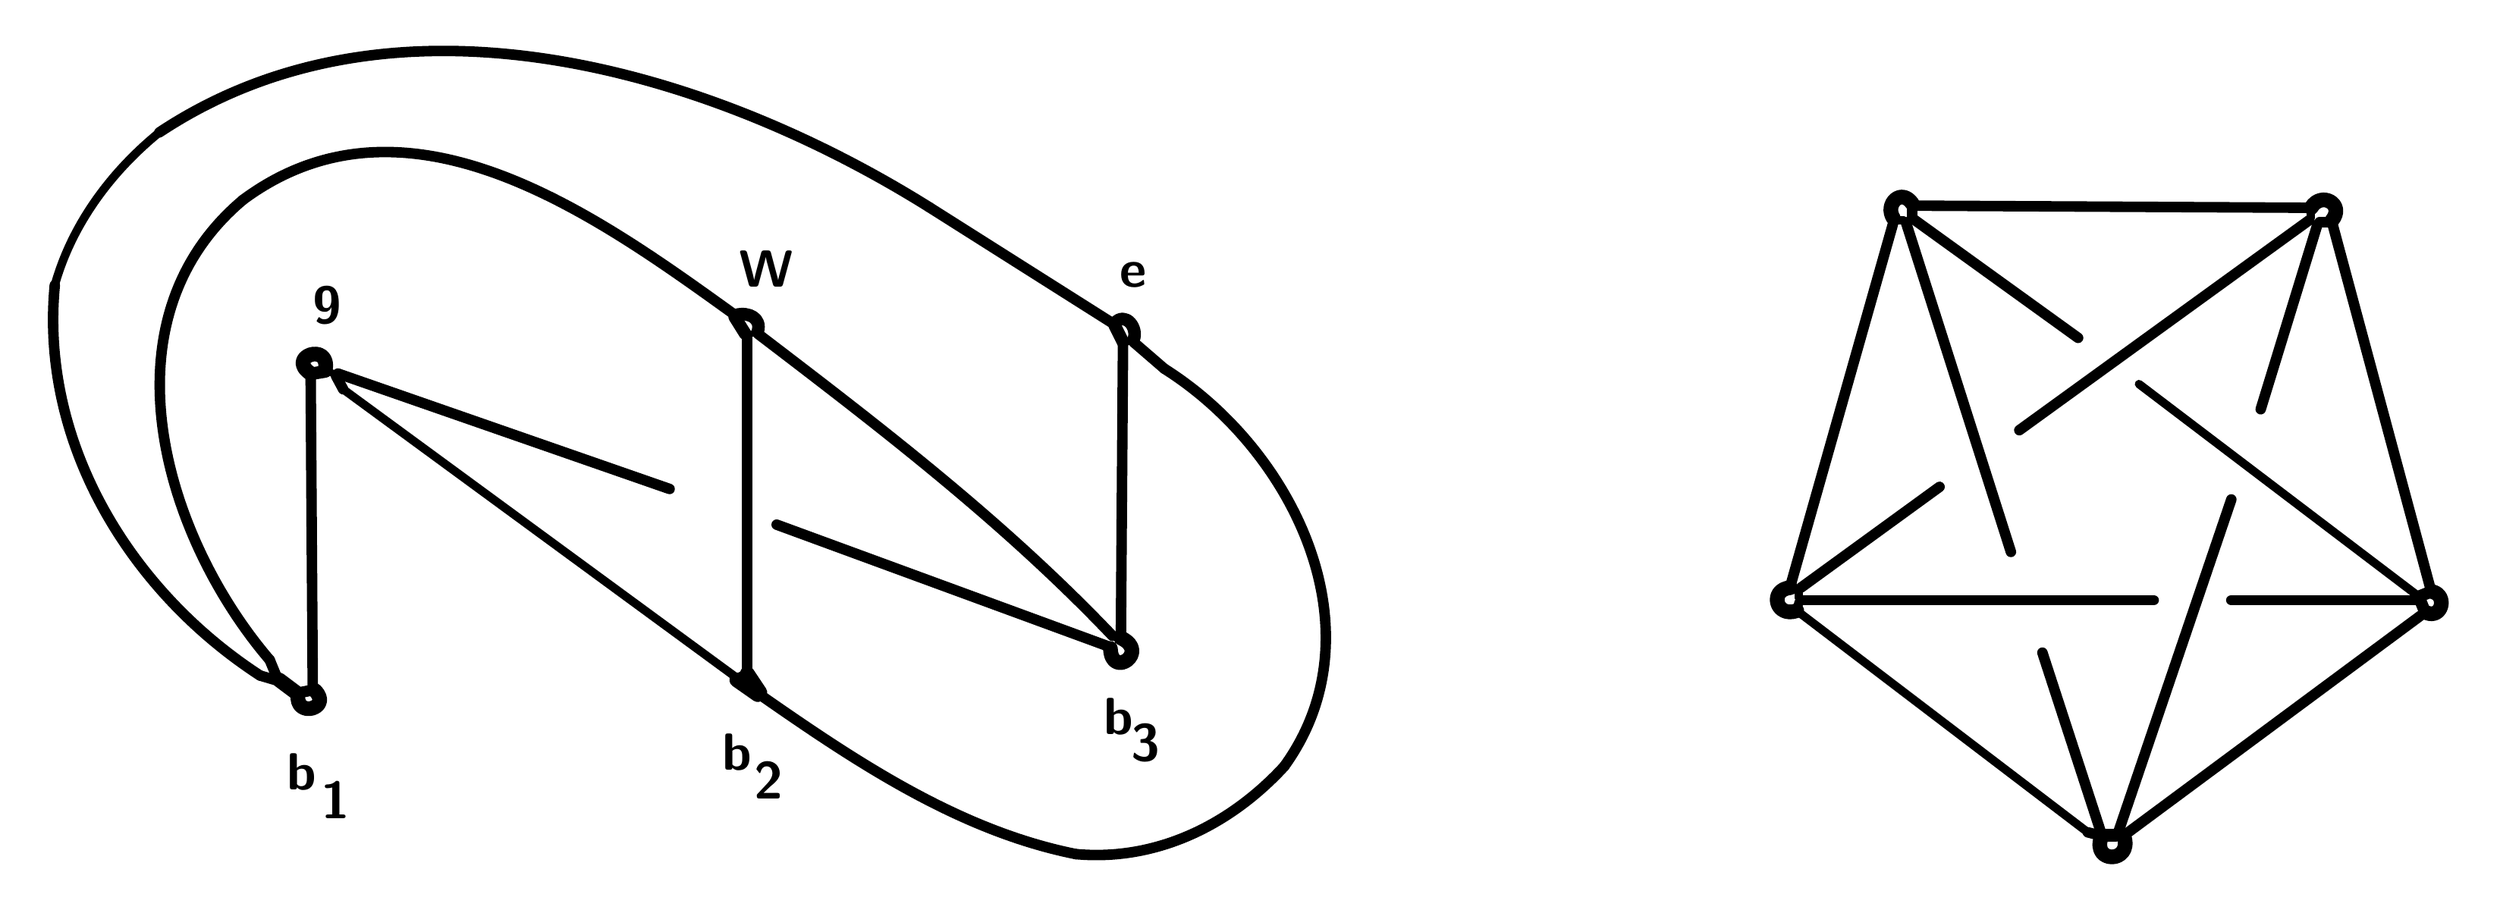
\begin{tikzpicture}[x=1pt, y=-1pt, line width=5.7pt, line cap=round, line join=round]

  %% ════ 直线段（prims2 的 strokes）════
  \draw[line width=5.7pt] (1148.0,272.0) -- (1143.0,274.0);
  \draw[line width=3.4pt] (146.0,167.0) -- (149.0,168.0);
  \draw[line width=5.0pt] (1094.0,97.0) -- (1067.0,185.0);
  \draw[line width=5.0pt] (1090.0,89.0) -- (902.0,88.0);
  \draw[line width=5.0pt] (848.0,270.0) -- (914.0,222.0);
  \draw[line width=4.0pt] (847.0,275.0) -- (847.0,271.0);
  \draw[line width=4.0pt] (1091.0,90.0) -- (1091.0,94.0);
  \draw[line width=5.0pt] (1090.0,95.0) -- (952.0,195.0);
  \draw[line width=3.0pt] (350.0,149.0) -- (347.0,149.0);
  \draw[line width=5.0pt] (848.0,276.0) -- (1016.0,276.0);
  \draw[line width=5.0pt] (999.0,387.0) -- (1053.0,228.0);
  \draw[line width=6.0pt] (998.0,388.0) -- (992.0,388.0);
  \draw[line width=5.0pt] (544.7,165.7) -- (530.0,153.0);
  \draw[line width=5.0pt] (1100.0,96.0) -- (1095.0,96.0);
  \draw[line width=5.0pt] (122.0,313.0) -- (118.5,304.5);
  \draw[line width=5.0pt] (138.0,169.0) -- (139.0,318.0);
  \draw[line width=5.7pt] (1143.0,276.0) -- (1145.0,281.0);
  \draw[line width=5.0pt] (892.0,96.0) -- (843.0,269.0);
  \draw[line width=4.0pt] (341.0,313.0) -- (153.5,175.5);
  \draw[line width=5.0pt] (153.5,175.5) -- (150.0,169.0);
  \draw[line width=6.0pt] (139.0,168.0) -- (145.0,167.0);
  \draw[line width=5.0pt] (520.0,144.0) -- (432.8,88.8);
  \draw[line width=5.0pt] (113.9,311.9) -- (121.0,314.0);
  \draw[line width=5.0pt] (980.0,151.0) -- (901.0,94.0);
  \draw[line width=4.0pt] (893.0,95.0) -- (897.0,95.0);
  \draw[line width=4.0pt] (1142.0,274.0) -- (1009.0,173.0);
  \draw[line width=6.0pt] (345.0,149.0) -- (340.0,141.0);
  \draw[line width=5.0pt] (948.0,253.0) -- (898.0,96.0);
  \draw[line width=5.0pt] (1002.0,388.0) -- (1145.0,282.0);
  \draw[line width=5.0pt] (346.0,150.0) -- (346.0,311.0);
  \draw[line width=6.0pt] (525.0,153.0) -- (521.0,145.0);
  \draw[line width=5.0pt] (1148.0,271.0) -- (1101.0,96.0);
  \draw[line width=7.0pt] (341.0,314.0) -- (351.0,321.0);
  \draw[line width=7.0pt] (131.0,320.0) -- (123.0,314.0);
  \draw[line width=5.0pt] (518.0,298.0) -- (360.0,240.0);
  \draw[line width=5.3pt] (133.0,320.0) -- (138.0,319.0);
  \draw[line width=5.0pt] (524.0,293.0) -- (525.0,154.0);
  \draw[line width=3.0pt] (529.0,153.0) -- (526.0,153.0);
  \draw[line width=7.0pt] (352.0,320.0) -- (346.0,311.0);
  \draw[line width=5.0pt] (901.0,89.0) -- (901.0,94.0);
  \draw[line width=5.0pt] (991.0,387.0) -- (963.0,301.0);
  \draw[line width=5.0pt] (990.0,388.0) -- (984.6,386.6);
  \draw[line width=4.0pt] (984.6,386.6) -- (846.0,281.0);
  \draw[line width=4.3pt] (847.0,277.0) -- (846.0,281.0);
  \draw[line width=5.0pt] (1053.0,276.0) -- (1141.0,276.0);
  \draw[line width=5.0pt] (309.0,223.0) -- (151.0,168.0);
  \draw[line width=4.7pt] (342.0,313.0) -- (346.0,311.0);

  %% ════ 曲线（prims2 的 curves —— 三段式，坐标同为 (y,x)）════
  \draw[line width=7.0pt] (901.0,87.0) .. controls (895.7,79.4) and (887.7,87.3) .. (892.0,94.0);
  \draw[line width=5.0pt] (520.0,293.0) .. controls (468.0,238.4) and (409.3,193.5) .. (351.0,149.0);
  \draw[line width=6.0pt] (351.0,148.0) .. controls (352.9,141.4) and (346.5,138.7) .. (341.0,140.0);
  \draw[line width=7.0pt] (524.0,294.0) .. controls (538.1,300.5) and (519.5,313.9) .. (519.0,299.0);
  \draw[line width=5.0pt] (352.0,321.0) .. controls (398.3,353.3) and (447.1,385.9) .. (502.6,397.0);
  \draw[line width=5.0pt] (502.6,397.0) .. controls (541.4,400.5) and (576.4,382.8) .. (601.8,355.2);
  \draw[line width=5.0pt] (601.8,355.2) .. controls (648.0,291.4) and (607.0,205.0) .. (544.7,165.7);
  \draw[line width=5.0pt] (118.5,304.5) .. controls (68.6,246.2) and (36.9,143.1) .. (105.8,85.2);
  \draw[line width=5.0pt] (105.8,85.2) .. controls (184.2,27.1) and (274.8,93.1) .. (340.0,140.0);
  \draw[line width=7.0pt] (1101.0,95.0) .. controls (1107.2,87.3) and (1095.8,80.9) .. (1091.0,89.0);
  \draw[line width=7.0pt] (843.0,270.0) .. controls (832.6,270.9) and (835.9,284.6) .. (846.0,281.0);
  \draw[line width=5.0pt] (432.8,88.8) .. controls (328.8,23.6) and (178.6,-21.8) .. (65.9,53.1);
  \draw[line width=4.0pt] (65.9,53.1) .. controls (42.0,72.6) and (24.0,97.7) .. (16.1,125.9);
  \draw[line width=5.0pt] (16.1,125.9) .. controls (8.9,200.7) and (51.6,271.4) .. (113.9,311.9);
  \draw[line width=7.0pt] (1146.0,282.0) .. controls (1153.4,284.9) and (1155.9,273.8) .. (1149.0,272.0);
  \draw[line width=7.0pt] (132.0,321.0) .. controls (130.4,332.4) and (148.6,327.6) .. (140.0,319.0);
  \draw[line width=7.0pt] (138.0,168.0) .. controls (126.1,160.0) and (147.2,152.8) .. (145.0,166.0);
  \draw[line width=7.0pt] (991.0,389.0) .. controls (986.6,401.7) and (1005.6,401.2) .. (1002.0,389.0);
  \draw[line width=6.0pt] (530.0,152.0) .. controls (532.4,146.2) and (526.1,138.2) .. (521.0,144.0);

  %% ════ 标签（probe 直接给的 \node 行）════
  %% ⚠ 全部补了 fill=white：文字在最上层，否则与曲线交叉干扰
     \node[anchor=center,inner sep=0pt,fill=white,font=\fontsize{23.6}{29.6}\selectfont] at (355.2,118.3) {\textsf{\textbf{\textit{W}}}};   % box(344,109,22,17)
     \node[anchor=center,inner sep=0pt,fill=white,font=\fontsize{31.4}{39.3}\selectfont] at (529.8,121.1) {\textsf{\textbf{\textit{e}}}};   % box(520,111,16,17)
     \node[anchor=center,inner sep=0pt,fill=white,font=\fontsize{34.8}{43.5}\selectfont] at (146.0,135.4) {\textsf{\textbf{9}}};   % box(135,123,18,23)
     \node[anchor=center,inner sep=0pt,fill=white,font=\fontsize{30.0}{37.5}\selectfont] at (522.8,331.2) {\textsf{\textbf{\textit{b}}}};   % box(513,319,17,22)
     \node[anchor=center,inner sep=0pt,fill=white,font=\fontsize{23.0}{28.7}\selectfont] at (535.9,344.1) {\textsf{\textbf{3}}};   % box(530,335,11,17)
     \node[anchor=center,inner sep=0pt,fill=white,font=\fontsize{30.9}{38.6}\selectfont] at (341.3,348.3) {\textsf{\textbf{\textit{b}}}};   % box(331,336,18,22)
     \node[anchor=center,inner sep=0pt,fill=white,font=\fontsize{30.7}{38.3}\selectfont] at (133.8,357.8) {\textsf{\textbf{\textit{b}}}};   % box(124,345,17,23)
     \node[anchor=center,inner sep=0pt,fill=white,font=\fontsize{23.6}{29.6}\selectfont] at (356.1,361.9) {\textsf{\textbf{2}}};   % box(350,353,11,17)
     \node[anchor=center,inner sep=0pt,fill=white,font=\fontsize{23.7}{29.7}\selectfont] at (149.8,371.4) {\textsf{\textbf{1}}};   % box(143,363,8,16)

  % 钉死画布：否则超出的图元/控制点会把页面撑大，1:1 回比就失准
  \pgfresetboundingbox
  \path[use as bounding box] (0,0) rectangle (1171,415);
\end{tikzpicture}
\end{document}

% ⚠ 待核清单（probe 拿不准，人眼过一遍）：
%   · 未识别/跳过：⑤ 跳过/未识别的字形
